%!TEX program = xelatex
\documentclass[tikz, border=0pt]{standalone} % 核心修改:改用standalone文档类
\usepackage[dvipsnames]{xcolor}
\usepackage{pgfplots}
\usepgfplotslibrary{colormaps,colorbrewer}
\pgfplotsset{compat=1.18}

\begin{document}
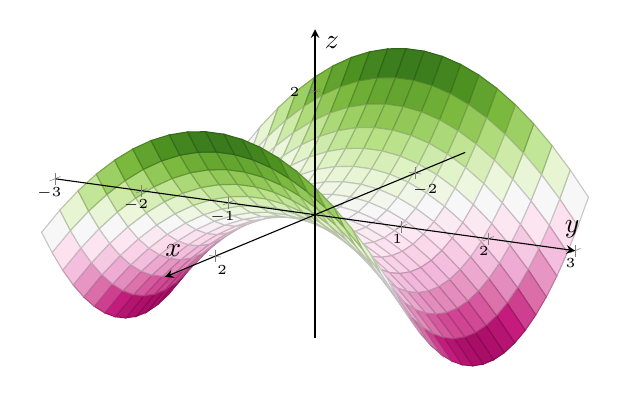
\begin{tikzpicture}
    \begin{axis}[
        tick label style={font=\tiny},
        view={120}{25},
        axis lines=center,
        axis on top,
        xlabel={$x$},ylabel={$y$},zlabel={$z$},
        xmin=-3,xmax=3, 
        ymin=-3,ymax=3,
        zmax=3,
        width=12cm,height=8cm
    ]
        \addplot3 [colormap/PiYG, surf, z buffer=sort, 
            samples=20, domain=-2:2, y domain=-2:2]
            ({x},{y},0.5*x^2-0.5*y^2);
    \end{axis}
\end{tikzpicture}
\end{document}
